\documentclass[aspectratio=169]{beamer}

%---------------------------
%       Beamer Cheat Sheet
%---------------------------
% https://www.cpt.univ-mrs.fr/~masson/latex/Beamer-appearance-cheat-sheet.pdf

%---------------------------
%       Set Theme and Colors
%---------------------------

\usetheme[width=.1\paperwidth]{Hannover}
% \setbeamertemplate{sidebar canvas right}[vertical shading][top=red,bottom=blue]

\definecolor{QESblue}{HTML}{8AD2ED}
\definecolor{QESdarkblue}{HTML}{187ca2}
\definecolor{QESlightblue}{HTML}{c4e8f6}

\setbeamercolor{sidebar}{bg=QESlightblue}
\setbeamercolor{titlelike}{fg=QESdarkblue}

\setbeamercolor{palette sidebar secondary}{fg=QESdarkblue}
\setbeamercolor{title in sidebar}{fg=QESdarkblue}
\setbeamercolor{author in sidebar}{fg=QESdarkblue}

\addtobeamertemplate{sidebar left}{}{\vfill \hspace{.006\paperwidth} 
\includegraphics[width=.08\paperwidth]{../../../logo.png} \vspace{.006\paperwidth} } 
% \addtobeamertemplate{sidebar left}{}{\vfill \hspace{.00001\paperwidth} 
\includegraphics[width=.093\paperwidth]{../../figures/qes-qr.png} \vspace{.003\paperwidth} } 

%---------------------------
%       No navigation symbols
%---------------------------
\setbeamertemplate{navigation symbols}{}

%---------------------------
%       Set Fonts
%---------------------------
\usepackage{helvet}
\renewcommand{\familydefault}{\sfdefault}
\usepackage{sansmathfonts}
\usepackage{upgreek}

\setbeamerfont{frametitle}{series=\bfseries, size=\Large}
\setbeamerfont{title in sidebar}{series=\bfseries, size=\small}
\setbeamertemplate{caption}{\it\raggedright\insertcaption\par}

%---------------------------
%       Math font packages
%---------------------------
\usepackage{dsfont, amsmath, amsthm, mathtools}
\usepackage{bbm, bm}
\usepackage[T1]{fontenc}
\usepackage[version=3]{mhchem}

%---------------------------
%       Figure packages
%---------------------------
\usepackage{graphicx}
\graphicspath{{../../figures}}

\usepackage{epstopdf}
\usepackage{color}

\setbeamerfont{caption}{size=\footnotesize}

\usepackage{subfigure}

%---------------------------
%       Manual placement packages
%---------------------------
\usepackage{tikz}
\usetikzlibrary{calc}

%---------------------------
%       Local Macros
%---------------------------

\newcommand{\manualpic}[4]{
    % inputs {filename}{figure options}{x offset}{y offset}
    \tikz[remember picture, overlay] \node[anchor=center] at ($(current page.center)+(#3,#4)$) {\includegraphics[#2]{#1}};
}

\newcommand{\manualtext}[3]{
    % inputs {text}{x offset}{y offset}
    \tikz[remember picture, overlay] \node[anchor=center] at ($(current page.center)+(#2,#3)$) {#1};
}

\newcommand{\manualtextleft}[3]{
    % inputs {text}{x offset}{y offset}
    \tikz[remember picture, overlay] \node[anchor=west] at ($(current page.center)+(#2,#3)$) {#1};
}

\newcommand{\manualtextright}[3]{
    % inputs {text}{x offset}{y offset}
    \tikz[remember picture, overlay] \node[anchor=east] at ($(current page.center)+(#2,#3)$) {#1};
}

\newcommand{\slidereference}[1]{
    \manualtextleft{\tiny #1}{-0.47\linewidth}{-0.47\textheight}
}

\newcommand{\dv}[2]{\frac{\mathrm{d}#1}{\mathrm{d}#2}}

\title{Ocean Carbon}
\author{5/5}

\begin{document}

\begin{frame}{Modelling the Oceans}
    
    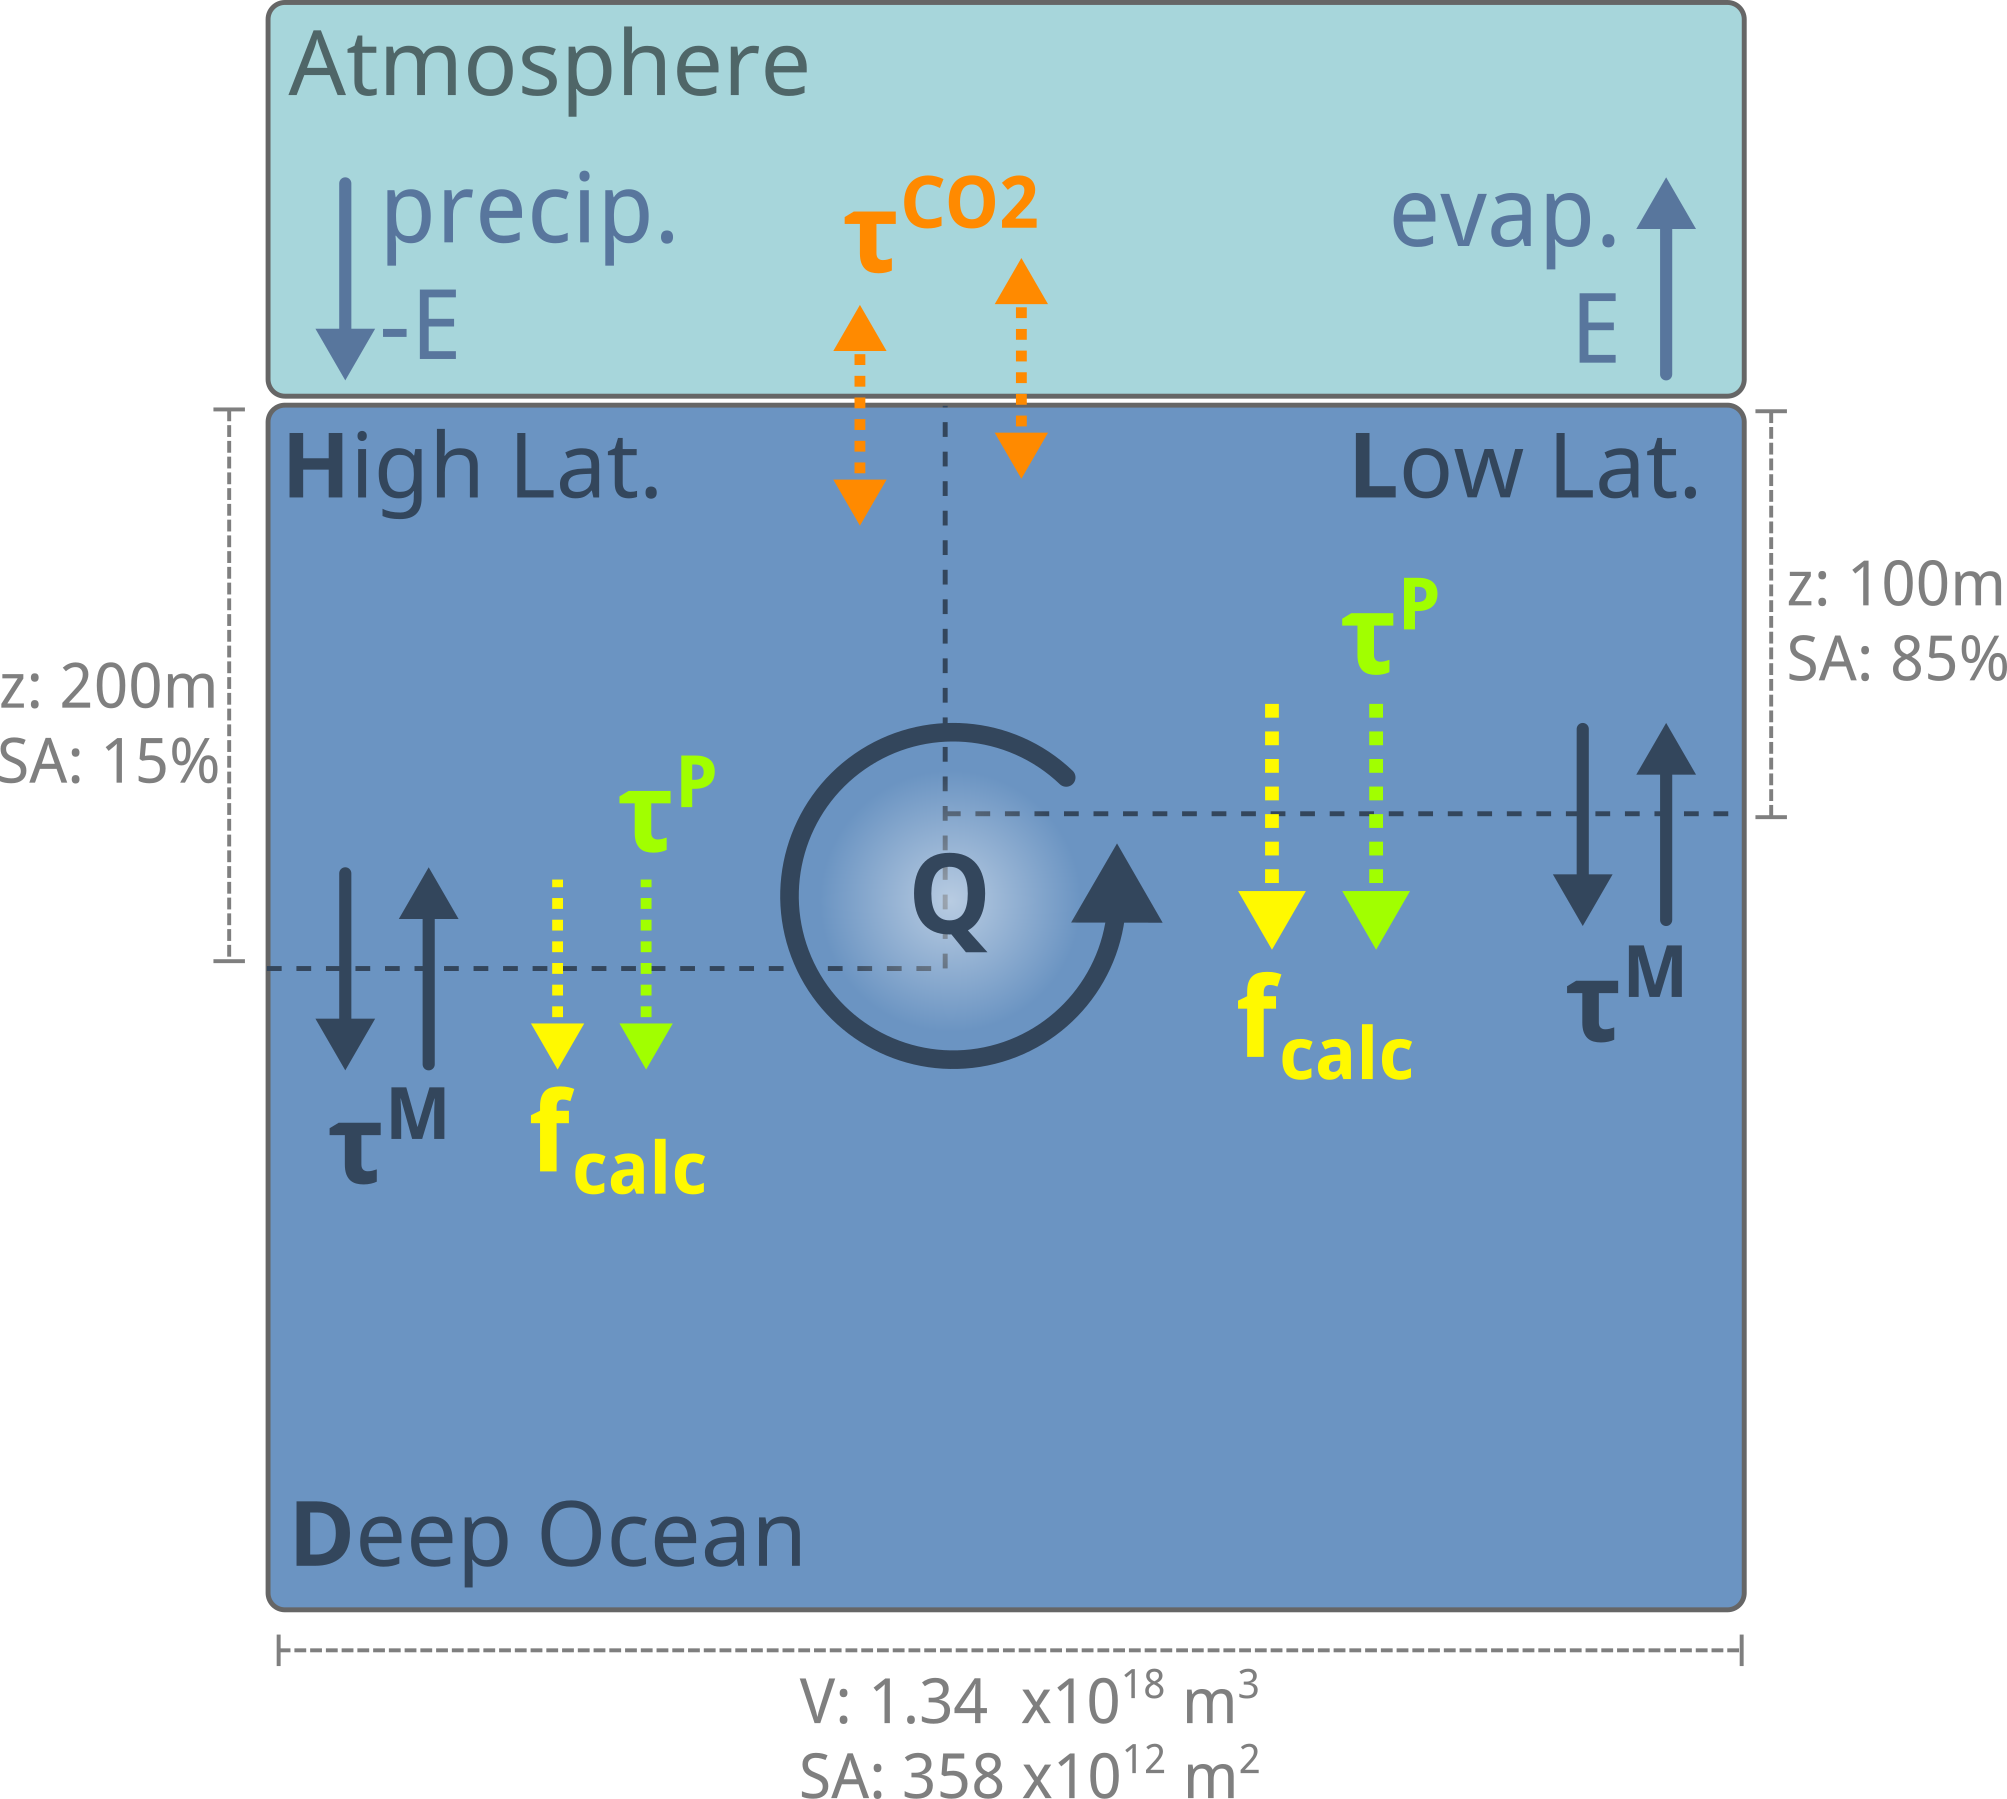
\includegraphics[width=\linewidth, totalheight=0.8\textheight, keepaspectratio]{ocean-3box-CO2-bio-calc-labels.png}
        
\end{frame}

\section{Practicalities}

\begin{frame}{Practicals and Lab Report}
    
    \begin{itemize}
        \item Answers to each practical will be accompanied by a short video to explain how the code works (first one tomorrow).
        \item An example lab report with a modified model will be released with P15 answers on (\textbf{2nd March}).
        \item Questions for the long section of the lab report will be released in P16 (\textbf{2nd March}).
        \item Practical drop-in sessions will continue until the end of term \textbf{March 16th}
        \item Lab report is due on \textbf{March 24th}.
        \item {\color{QESdarkblue}We will go through the structure and logic of the model code today.}
    \end{itemize}
        
\end{frame}

\section{Model Code}

\begin{frame}{Model Code}
    \includegraphics<1>[width=\linewidth, height=0.8\textheight, keepaspectratio]{carbon-model-TS.png}
\end{frame}

\section{Model Parameters}

\begin{frame}<handout:0>{Model Parameters}
    
    Forcing:
    \begin{itemize}
        \item Atmospheric Temperature
        \item Evaporation/Precipitation
    \end{itemize}

    \onslide<2>{
        Processes:
        \begin{itemize}
            \item $\tau^M$ - Surface-Deep Mixing
            \item $\tau^T$ - Atmosphere-Surface Temperature Equilibration
            \item $\tau^{CO2}$ - Atmosphere-Surface CO$_2$ Equilibration
            \item $\tau^P$ - Nutrient Uptake by Phytoplankton
            \item Redfield ratio - Composition of Organic Matter
            \item $f_{CaCO3}$ - Fraction of CaCO$_3$ associated with Organic Matter
        \end{itemize}
    }

\end{frame}

\section{State Dependence?}

\begin{frame}{Model Parameters}
    
    Forcing:
    \begin{itemize}
        \item Atmospheric Temperature - {\color{QESdarkblue} \ce{CO2}?}
        \item Evaporation/Precipitation - {\color{QESdarkblue} Temperature? Wind?}
    \end{itemize}

    Processes:
    \begin{itemize}
        \item $\tau^M$ - Surface-Deep Mixing - {\color{QESdarkblue} Eddies? Stratification? Storms?}
        \item $\tau^T$ - Atmosphere-Surface Temperature Equilibration - {\color{QESdarkblue} Mixing? Wind?}
        \item $\tau^{CO2}$ - Atmosphere-Surface CO$_2$ Equilibration - {\color{QESdarkblue} Mixing? Wind?}
        \item $\tau^P$ - Nutrient Uptake by Phytoplankton - {\color{QESdarkblue} Ecology?}
        \item Redfield ratio - Composition of Organic Matter - {\color{QESdarkblue} Ecology?}
        \item $f_{CaCO3}$ - Fraction of CaCO$_3$ associated with Organic Matter - {\color{QESdarkblue} \ce{\Omega}?}
    \end{itemize}

\end{frame}

\begin{frame}{Model Complexity}
    \centering
    \includegraphics<1>[width=\linewidth, totalheight=0.6\textheight, keepaspectratio]{model-resolution.jpg}
    \includegraphics<2>[width=\linewidth, totalheight=0.8\textheight, keepaspectratio]{model-processes.jpg}
    \slidereference{CarbonBrief}
\end{frame}

\begin{frame}{Ocean Acidification}
    
    Forcing:
    \begin{itemize}
        \item Atmospheric Temperature - {\color{QESdarkblue} \ce{CO2}?}
        \item Evaporation/Precipitation - {\color{QESdarkblue} Temperature? Wind?}
    \end{itemize}

    Processes:
    \begin{itemize}
        \item $\tau^M$ - Surface-Deep Mixing - {\color{QESdarkblue} Stratification? Storms?}
        \item $\tau^T$ - Atmosphere-Surface Temperature Equilibration - {\color{QESdarkblue} Mixing? Wind?}
        \item $\tau^{CO2}$ - Atmosphere-Surface CO$_2$ Equilibration - {\color{QESdarkblue} Mixing? Wind?}
        \item $\tau^P$ - Nutrient Uptake by Phytoplankton - {\color{QESdarkblue} Ecology?}
        \item Redfield ratio - Composition of Organic Matter - {\color{QESdarkblue} Ecology?}
        \item {\color{red}${f_{CaCO3}}$ \textbf{- Fraction of CaCO$_3$ associated with Organic Matter - {\color{QESdarkblue} \ce{\Omega}?}}}
    \end{itemize}

\end{frame}

\section{Ocean Acidification}

\begin{frame}{Modelling Ocean Acidification}
    $\mathbf{f_{CaCO3}}$ \textbf{- Fraction of CaCO$_3$ associated with Organic Matter - {\color{QESdarkblue} \ce{\Omega}?}}
    
    \bigskip
    \begin{columns}
        \begin{column}{0.5\linewidth}
            \centering
            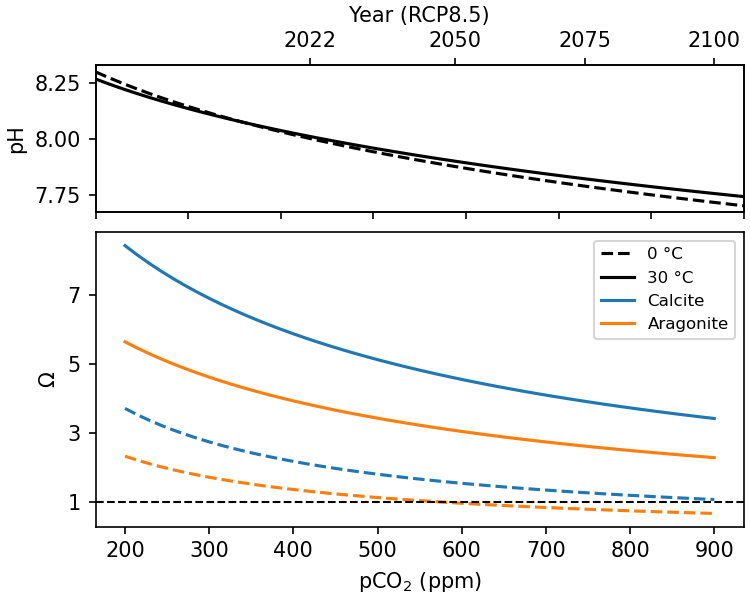
\includegraphics[width=\linewidth, keepaspectratio]{carbon-pCO2-pH.png}
        \end{column}
        \begin{column}{0.5\linewidth}
            \begin{align*}
                \ce{[CO3^{2-}]} &\varpropto \ce{pCO2}\\
                \Omega &= \frac{\ce{[Ca^{2+}][CO3^{2-}]}}{K_{sp}} \\
                f_{CaCO3} &= g(\Omega) \\
            \end{align*}
            
        \end{column}
    \end{columns}
\end{frame}

\begin{frame}{Modelling Ocean Acidification}
    \begin{enumerate}
        \item \ce{CaCO3} Production
        \item \ce{CacO3} Dissolution
    \end{enumerate}
\end{frame}

\subsection{Production}

\begin{frame}{Production}
    \begin{columns}
        \begin{column}{0.45\linewidth}
            \centering
            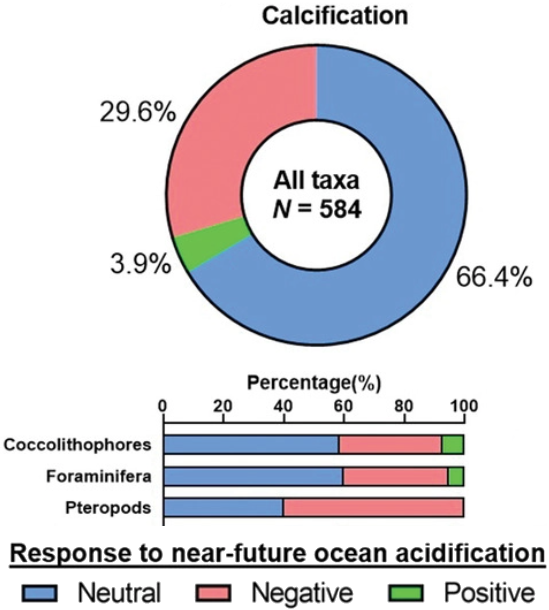
\includegraphics[width=\linewidth, keepaspectratio]{carbon-calcification-response.png}
        \end{column}
        \begin{column}{0.55\linewidth}
            $$f_{production} = g(\Omega)$$
        \end{column}
    \end{columns}
    \slidereference{Leung et al. (2022)}
\end{frame}

\begin{frame}<handout:0>{Production}
    \begin{columns}
        \begin{column}{0.45\linewidth}
            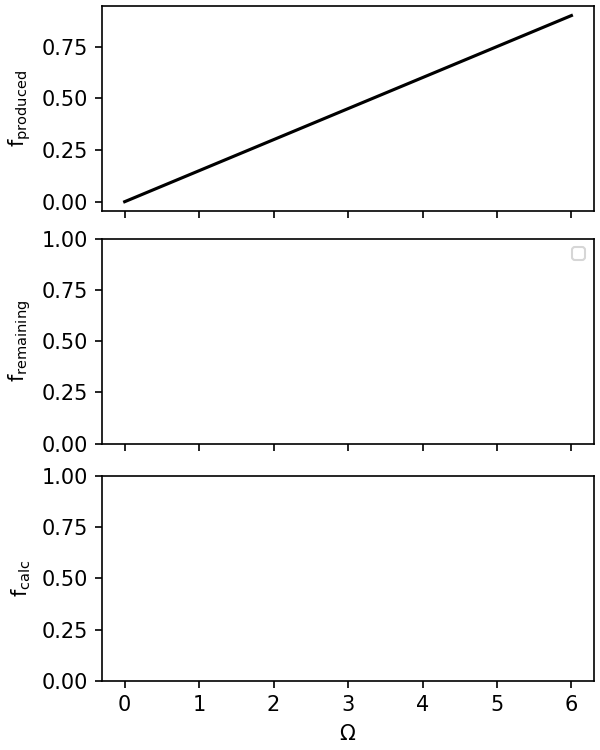
\includegraphics[width=\linewidth, keepaspectratio]{ocean-3box-f_calc.0.png}
        \end{column}
        \begin{column}{0.55\linewidth}
            $$f_{production} = 0.15 \Omega$$
        \end{column}
    \end{columns}
\end{frame}

\subsection{Dissolution}

\begin{frame}{Dissolution: Inorganic}
    \begin{columns}
        \begin{column}{0.45\linewidth}
            \centering
            \includegraphics<1|handout:0>[width=\linewidth, height=0.8\textheight, keepaspectratio]{carbonate-dissolution-rate.0.png}
            \includegraphics<2|handout:0>[width=\linewidth, height=0.8\textheight, keepaspectratio]{carbonate-dissolution-rate.1.png}
            \includegraphics<3|handout:1>[width=\linewidth, height=0.8\textheight, keepaspectratio]{carbonate-dissolution-rate.2.png}
        \end{column}
        \begin{column}{0.55\linewidth}
            \only<2-|handout:0>{
                $$f_{remaining} = e^{k t (1 - \Omega)^n}$$
            }
        \end{column}
    \end{columns}
\end{frame}

\begin{frame}{Dissolution: Ocean}
    \begin{columns}
        \begin{column}{0.45\linewidth}
            \centering
            \includegraphics<1|handout:1>[width=\linewidth, height=0.8\textheight, keepaspectratio]{carbon-caco3-flux.png}
            \includegraphics<2|handout:0>[width=\linewidth, height=0.8\textheight, keepaspectratio]{carbon-CO3-sat-real.png}
            \includegraphics<3|handout:2>[width=\linewidth, height=0.8\textheight, keepaspectratio]{carbon-caco3-dissolution.png}
            \includegraphics<4|handout:3>[width=\linewidth, height=0.8\textheight, keepaspectratio]{carbon-omega-met.png}
        \end{column}
        \begin{column}{0.55\linewidth}
            \only<1-3|handout:1-2>{
                $$f_{remaining} = e^{k t (1 - \Omega)^n}$$
            }
            \only<4|handout:3>{
                $$f_{remaining} = e^{k t ({\color{red}\Omega_{crit}} - \Omega)^n}$$
                $$\Omega_{crit} \approx 3 $$
            }

        \end{column}
    \end{columns}
    \only<1-3|handout:1-2>{\slidereference{Sulpis et al. (2021)}}
    \only<4|handout:3>{\slidereference{Subhas et al. (2022)}}
\end{frame}

\begin{frame}{Dissolution}
    \begin{columns}
        \begin{column}{0.45\linewidth}
            \centering
            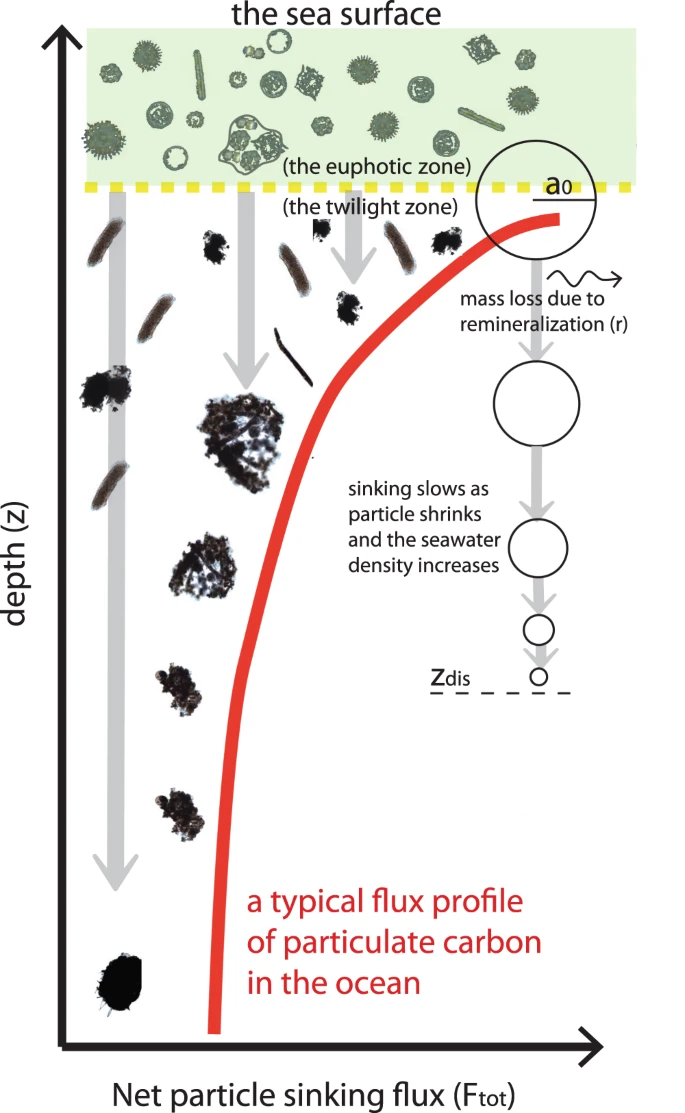
\includegraphics[width=\linewidth, height=0.8\textheight, keepaspectratio]{carbon-particle-sinking.png}
        \end{column}
        \begin{column}{0.55\linewidth}
            $$f_{remaining} = e^{k {\color{red}\frac{z}{s}} (\mathbf{\Omega_{crit}} - \Omega)^n}$$
            $$s \approx 10~m~s^{-1}$$
        \end{column}
    \end{columns}

    \slidereference{Omand et al. (2020)}
\end{frame}

\begin{frame}{Dissolution}
    \begin{columns}
        \begin{column}{0.45\linewidth}
            \centering
            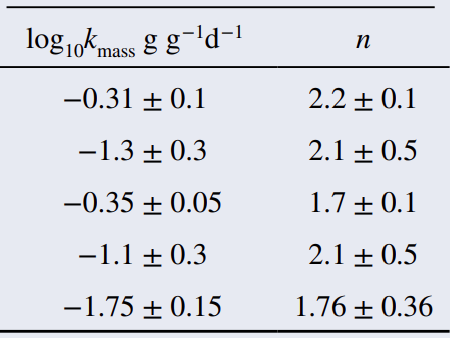
\includegraphics[width=0.6\linewidth, height=0.8\textheight, keepaspectratio]{carbon-calc-dissolutionparams.png}
        \end{column}
        \begin{column}{0.55\linewidth}
            $$f_{remaining} = e^{{\color{red}k} \frac{z}{s} (\mathbf{\Omega_{crit}} - \Omega)^{\color{red}n}}$$
            \begin{align*}
                k & \approx 10^{-1.75} - 10^{-0.3} \\
                & \approx 0.02 - 0.50
            \end{align*}
            $$n \approx 2$$
        \end{column}
    \end{columns}

    \slidereference{Subhas et al. (2022)}
\end{frame}

\begin{frame}{Dissolution}
    \begin{columns}
        \begin{column}{0.45\linewidth}
            \centering
            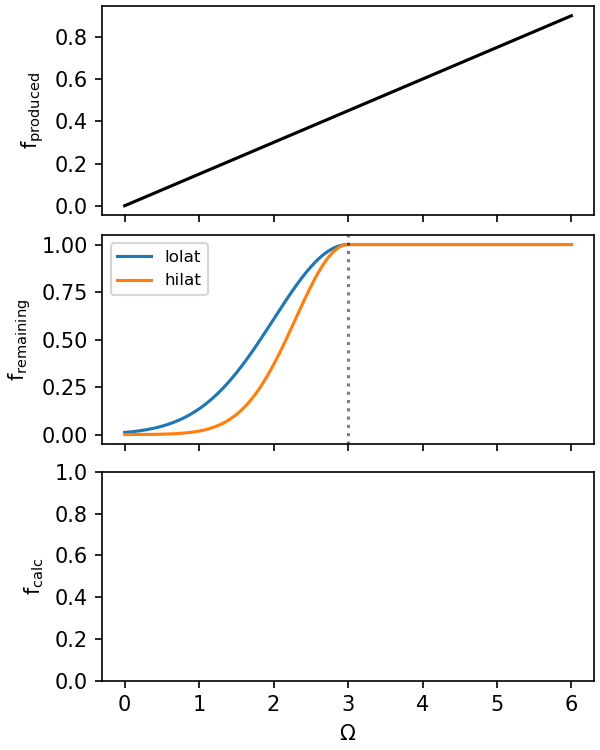
\includegraphics[width=\linewidth, keepaspectratio]{ocean-3box-f_calc.1.png}
        \end{column}
        \begin{column}{0.55\linewidth}
            $$f_{remaining} = \begin{cases}
                e^{k \frac{z}{s} (\mathbf{\Omega_{crit}} - \Omega)^n} & \Omega < \Omega_{crit} \\
                1 & \Omega \geq \Omega_{crit}
            \end{cases}
            $$
        \end{column}
    \end{columns}
\end{frame}

\subsection{Export}

\begin{frame}{Export}
    \begin{columns}
        \begin{column}{0.45\linewidth}
            \centering
            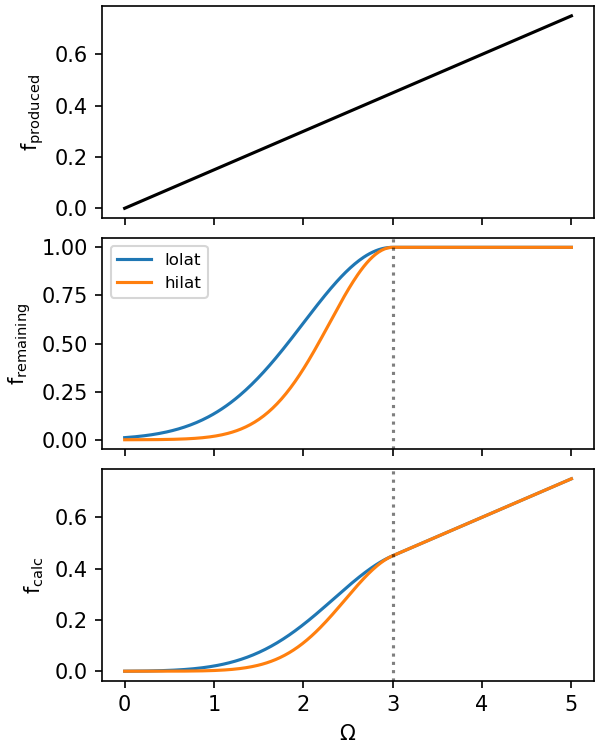
\includegraphics[width=\linewidth, keepaspectratio]{ocean-3box-f_calc.2.png}
        \end{column}
        \begin{column}{0.55\linewidth}
            \begin{align*}
                f_{CaCO3} &= f_{production} ~ f_{remaining} \\
                f_{CaCO3} &= \begin{cases}
                    0.15 \Omega e^{k \frac{z}{s} (\mathbf{\Omega_{crit}} - \Omega)^n} & \Omega < \Omega_{crit} \\
                    0.15 \Omega & \Omega \geq \Omega_{crit}
                \end{cases}
            \end{align*}
        \end{column}
    \end{columns}
\end{frame}

\section{Results}

\subsection{Steady State}

\begin{frame}{Steady State}
    \centering
    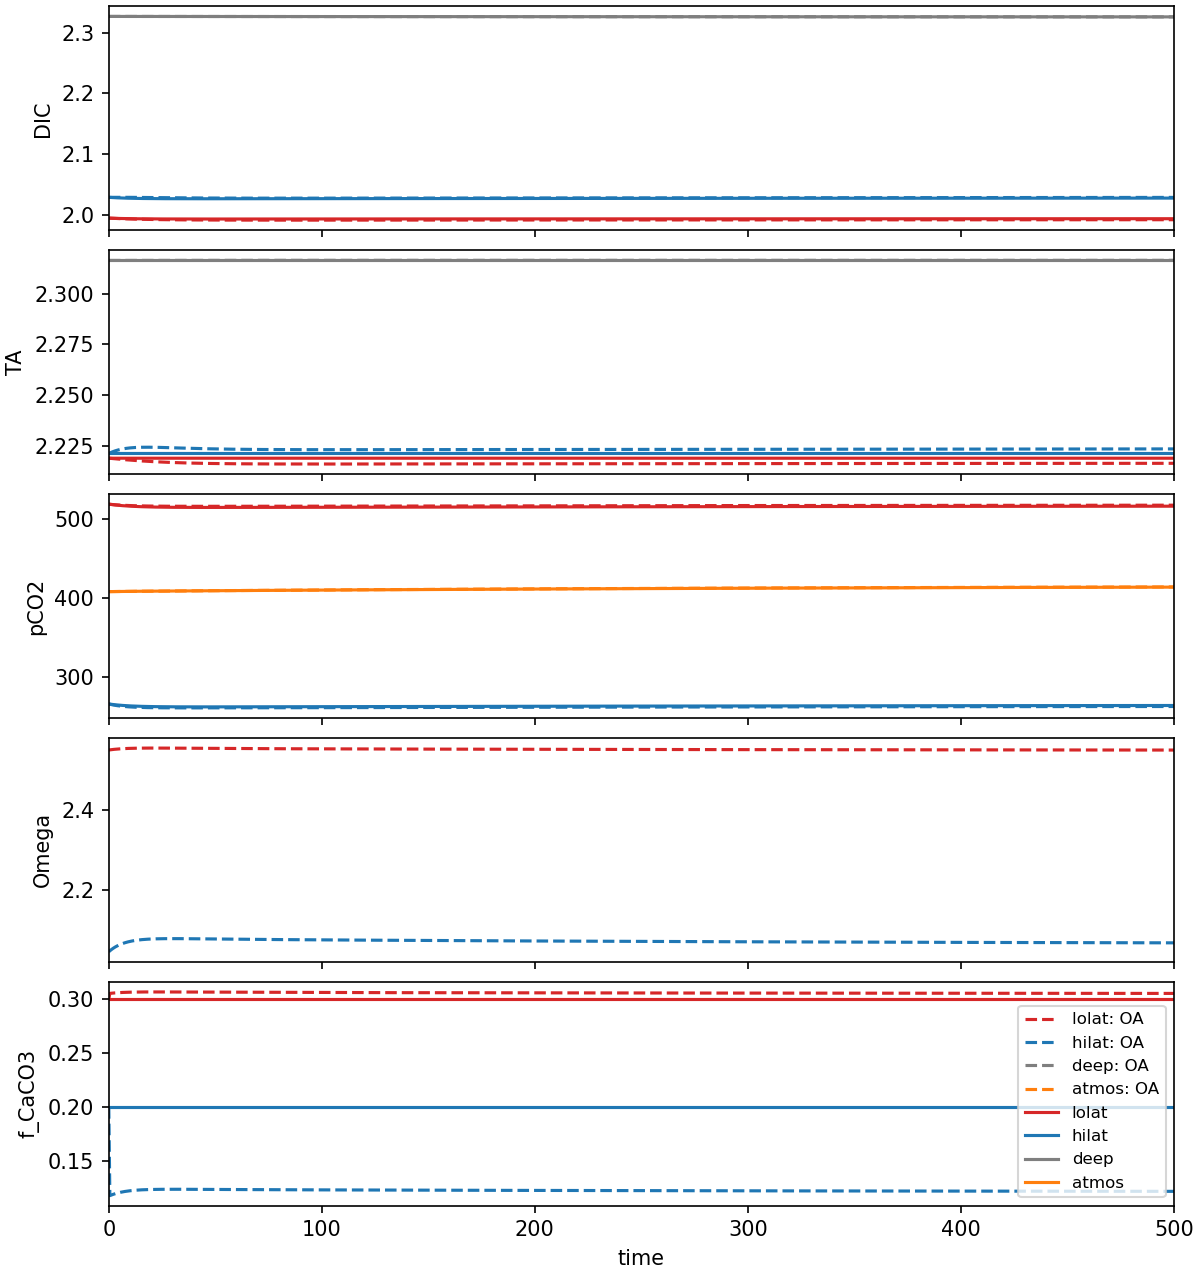
\includegraphics[width=\linewidth, totalheight=0.8\textheight, keepaspectratio]{ocean-3box-OA-SS.png}

\end{frame}

\subsection{\ce{CO2} Release}

\begin{frame}{\ce{CO2} Release}
    \centering
    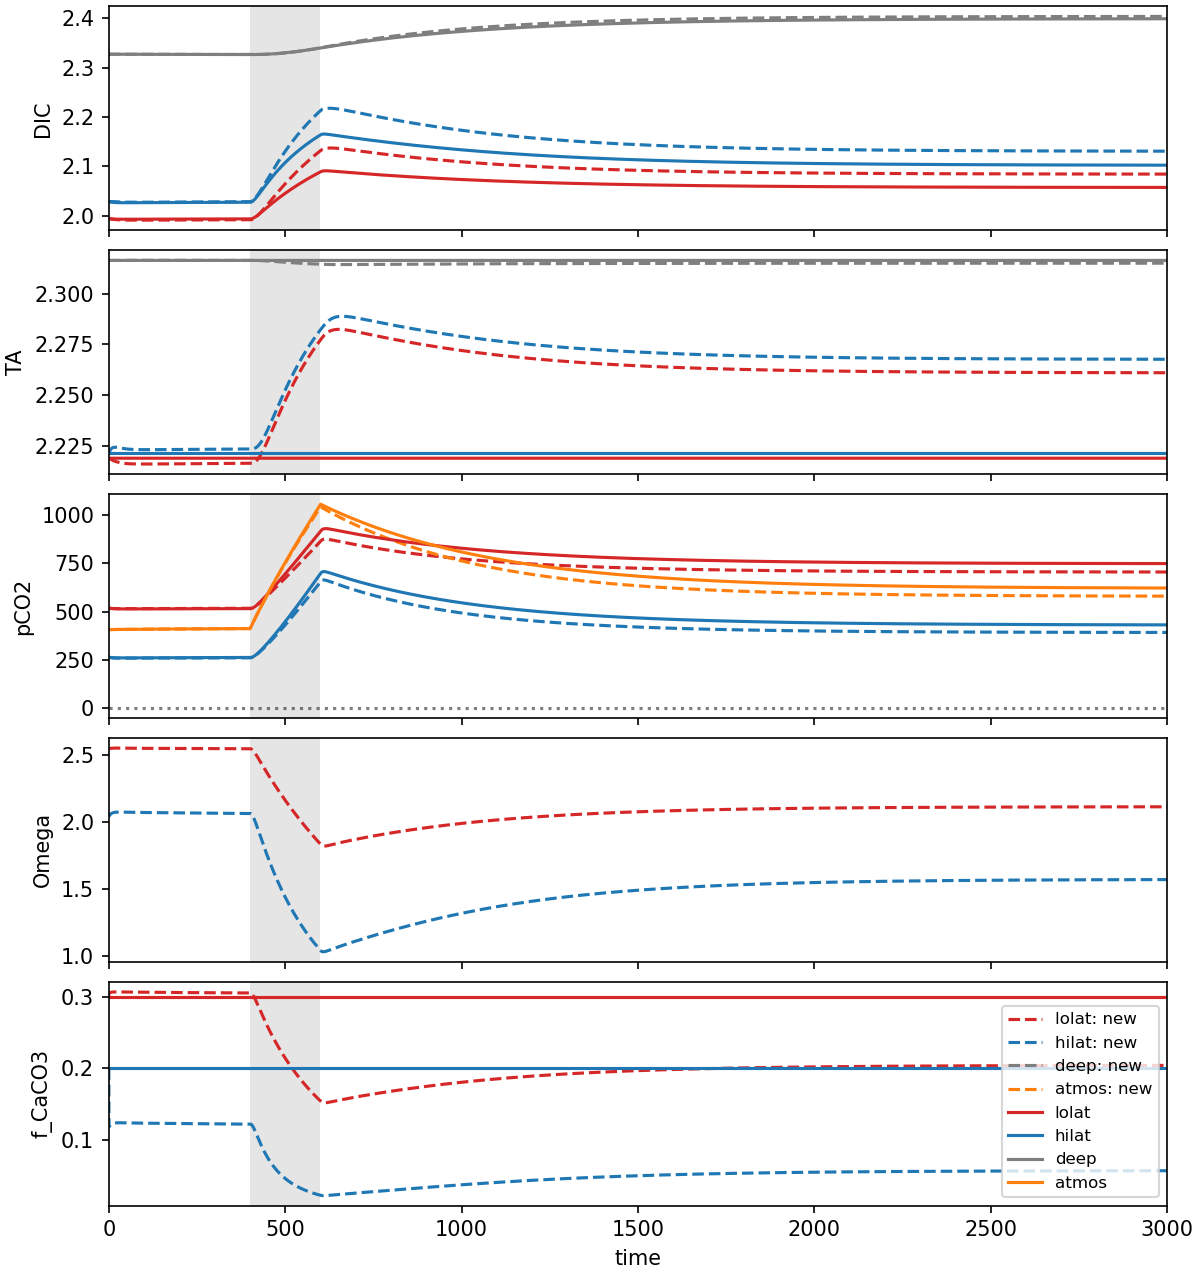
\includegraphics[width=\linewidth, totalheight=0.8\textheight, keepaspectratio]{ocean-3box-OA-CO2-release.png}
\end{frame}

\begin{frame}{\ce{CO2} Release}
    \centering
    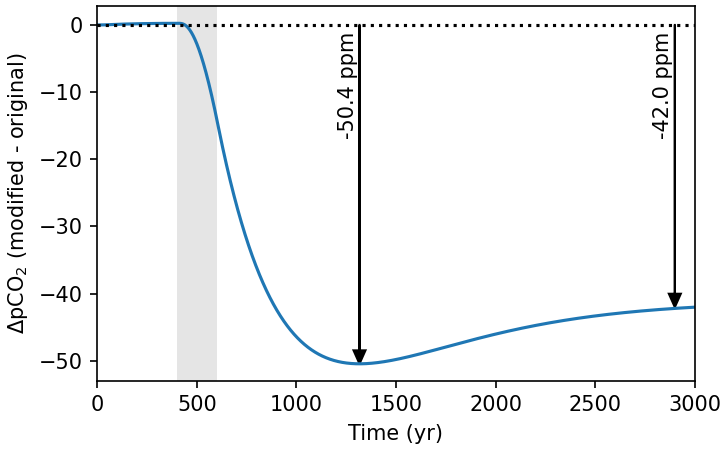
\includegraphics[width=\linewidth, totalheight=0.6\textheight, keepaspectratio]{ocean-3box-OA-CO2-comparison.png}
\end{frame}

\subsection{Other Factors}

\begin{frame}{(Bio)Mineralogy}
    \centering
    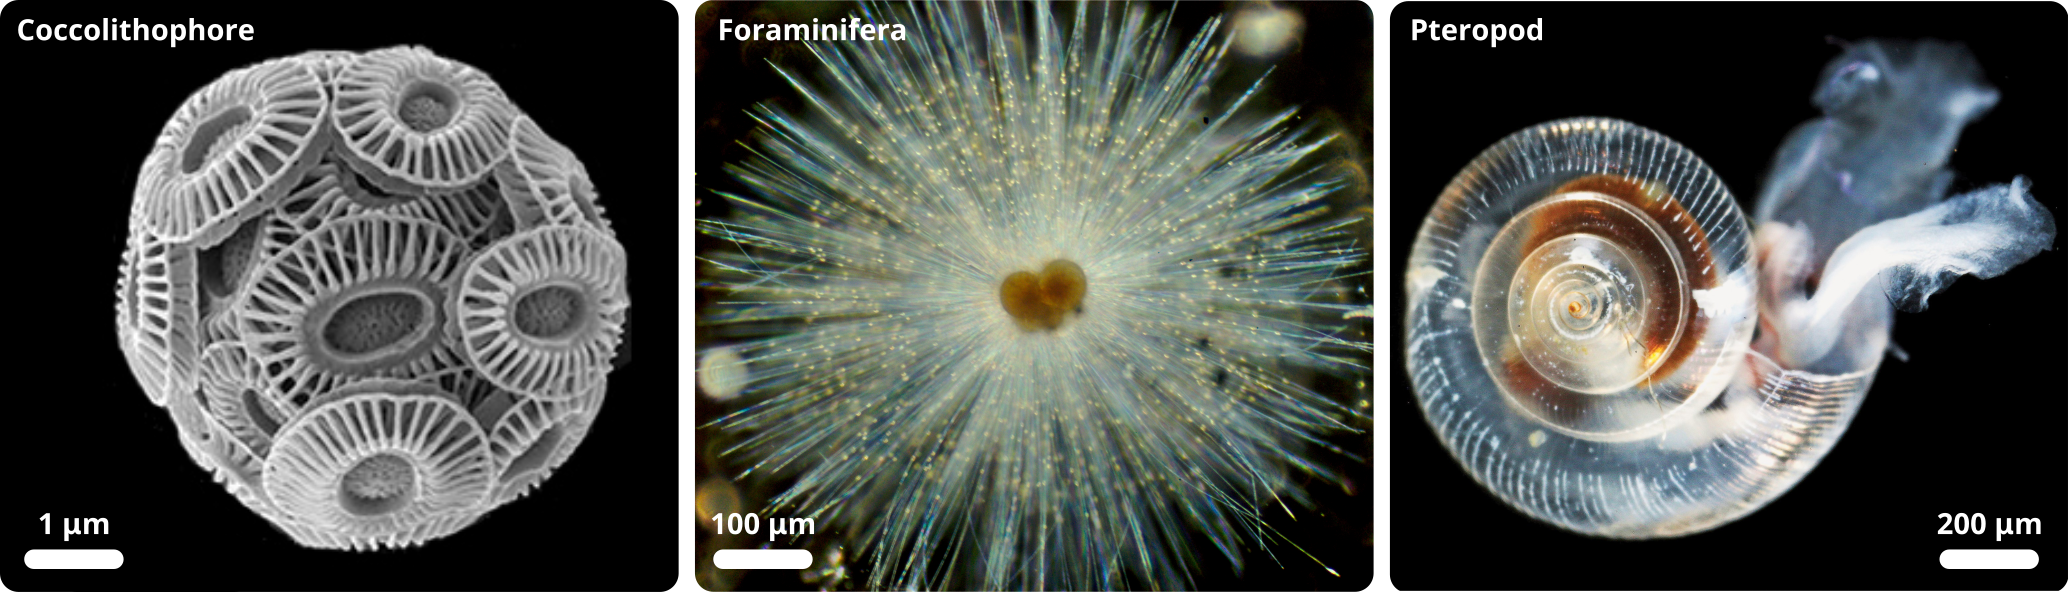
\includegraphics[width=\linewidth, totalheight=0.8\textheight, keepaspectratio]{carbon-calcifiers.png}

\end{frame}

\begin{frame}{Ballasting}
    \centering
    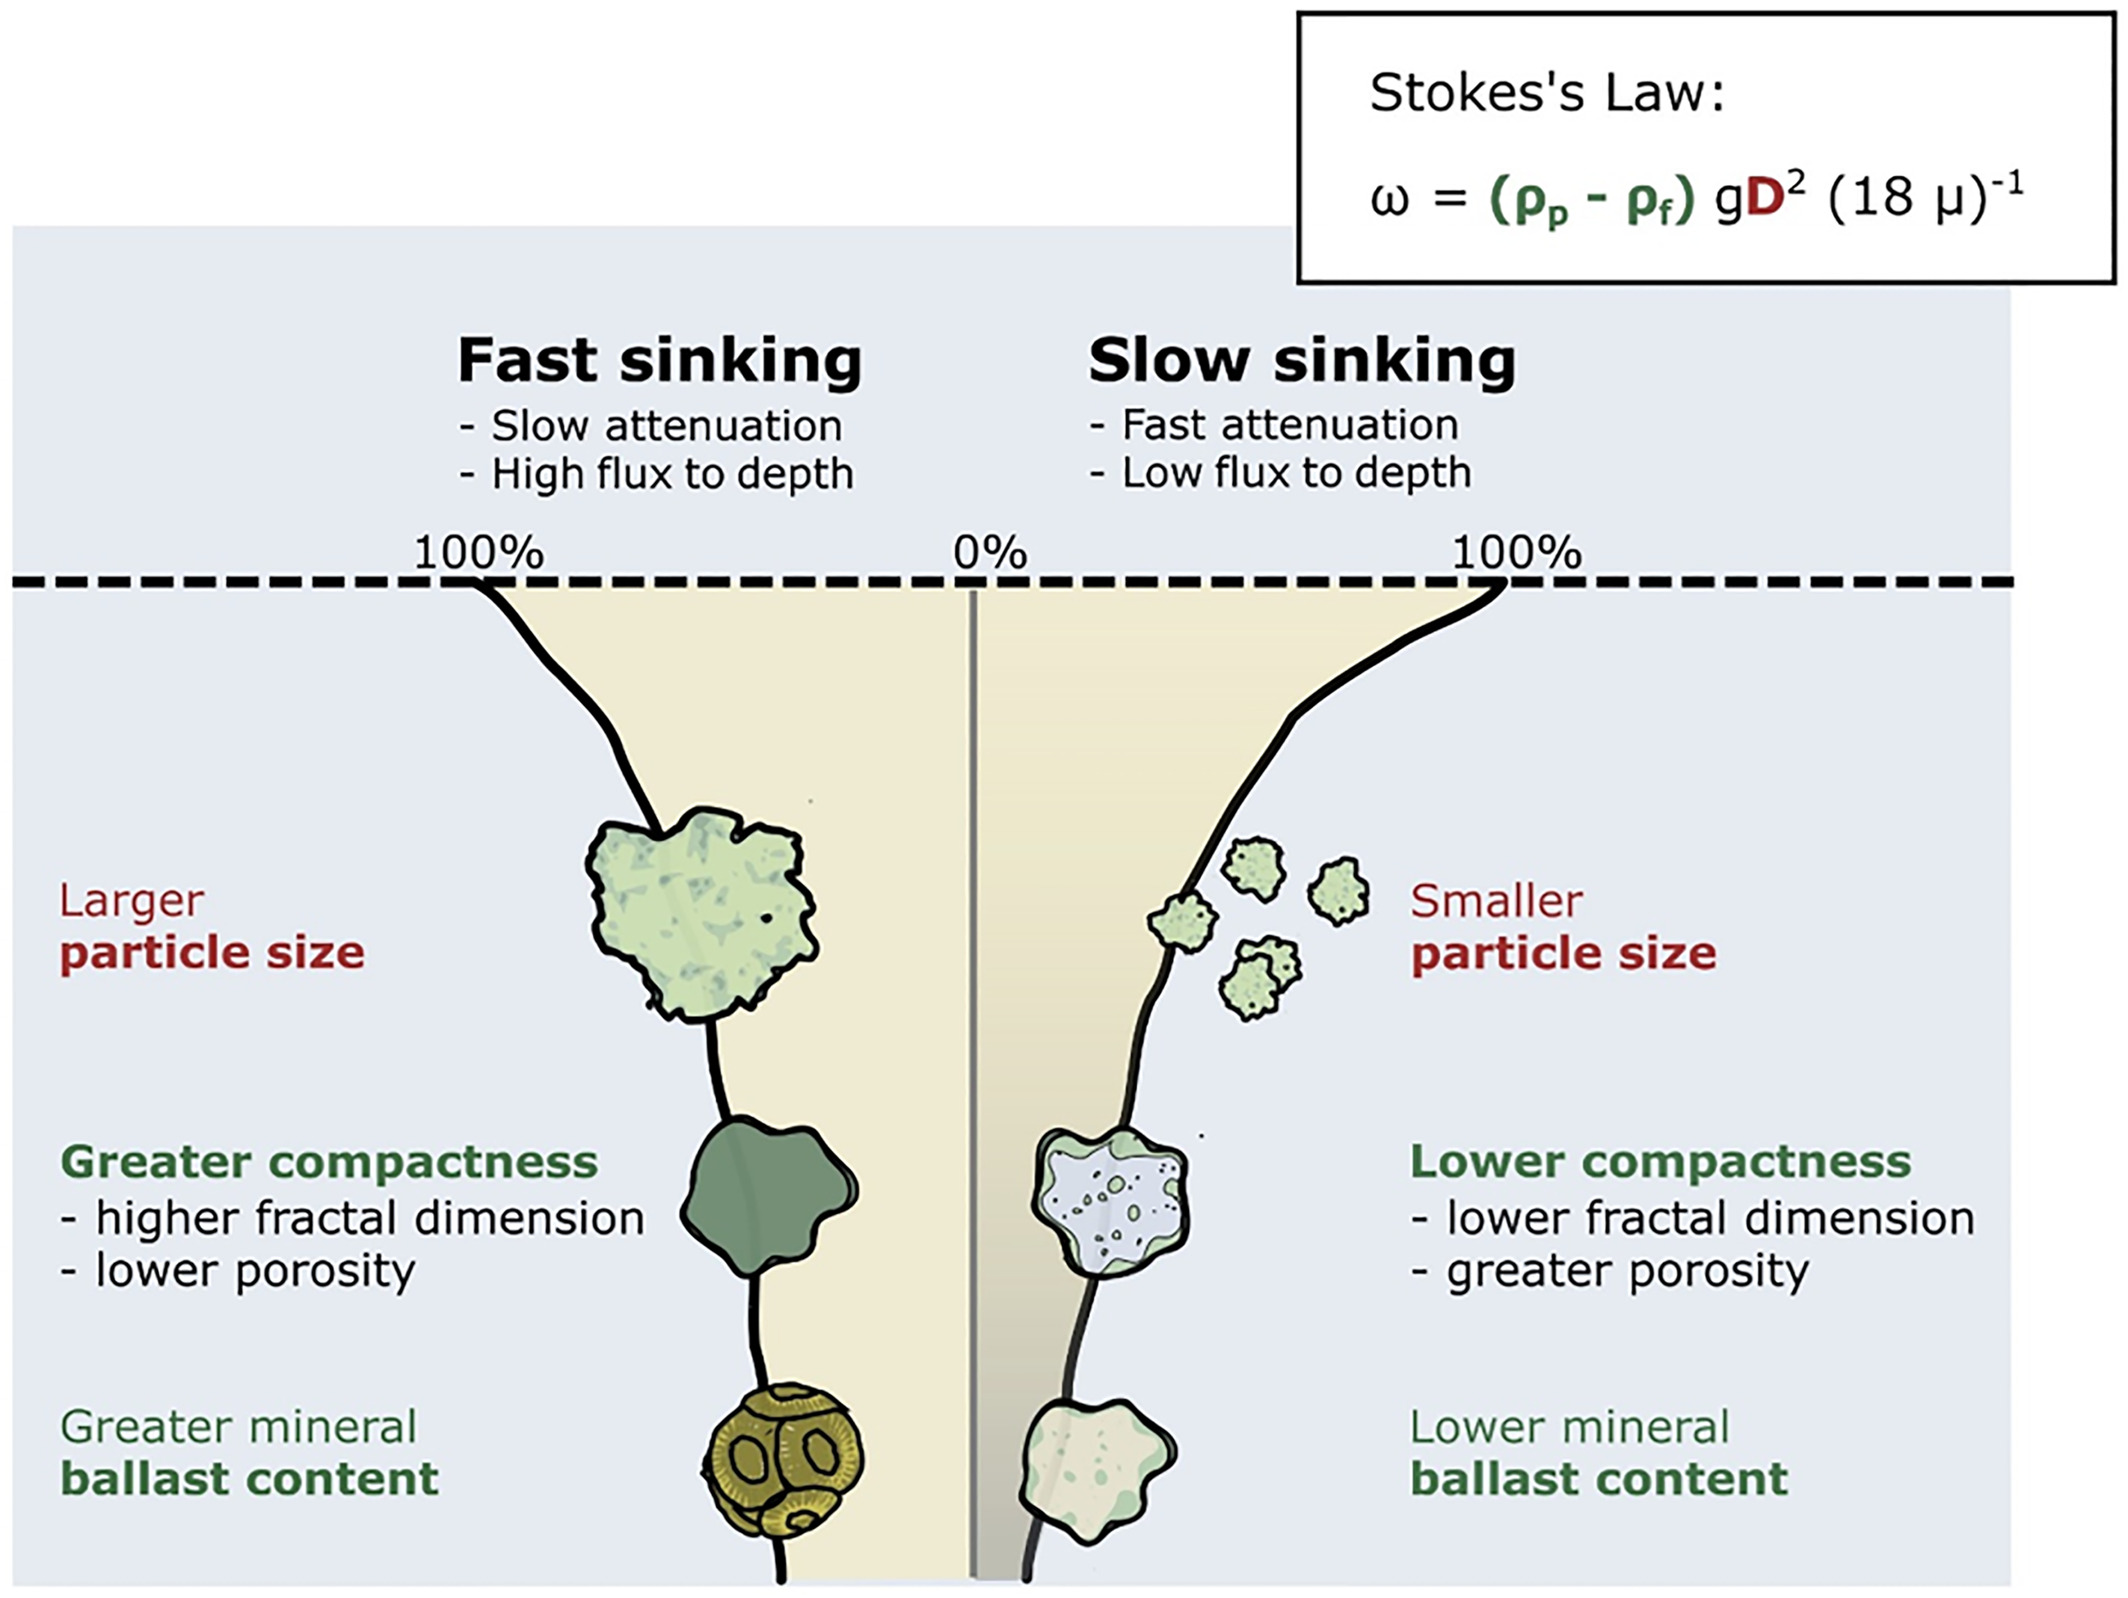
\includegraphics[width=\linewidth, totalheight=0.8\textheight, keepaspectratio]{carbon-particle-flux.jpg}

\end{frame}

\end{document}





% \begin{frame}{TITLE}
% \end{frame}